\documentclass{article}
%
\usepackage{hevea}
%
\usepackage{url}
%
\usepackage{ifpdf}
%
%TODO: Define this command only when hevea is run not pdflatex.
\newcommand{\includegraphics}[1]{\imgsrc{#1.png}}
%
\newcommand\codspec{CodingSpectator}
%
\newcommand\warnnote[1]{\textbf{Note: }#1}
%
\newcommand\infonote[1]{\textbf{Note: }#1}
%
\newcommand\uiref[1]{"\texttt{#1}"}
%
\title{\codspec's User Guide}
%
\author{\codspec\ Team\\codingspectator@gmail.com}
%
\begin{document}
%
\maketitle
%
\tableofcontents
%
\section{Prerequisites}
%
You should be using Eclipse 3.6 Helios. You may check which version you have
installed by looking at the logo that appears during startup; it should say
Eclipse Helios.

\warnnote{Please note that the plug-in cannot be installed on an older version
of Eclipse e.g. Eclipse 3.5 Ganymede. It only works with Eclipse 3.6 Helios. If
you are using Helios but are still having problems please contact us.}
%
\section{Installing our plug-in}

After installing Eclipse, you need to install our plug-in by following the steps
below:

\begin{enumerate}
%
\item In Eclipse, go to \uiref{Help > Install New Software...}.
%
\item Click the \uiref{Add} button on the top right corner of the dialog.
%
\item Add a new update-site. Set the \uiref{Name} to \codspec\ and the
\uiref{Location} to \url{http://codingspectator.cs.illinois.edu/updates} as
shown below. Then, click \uiref{OK}.

\begin{figure}
%
\centering
%
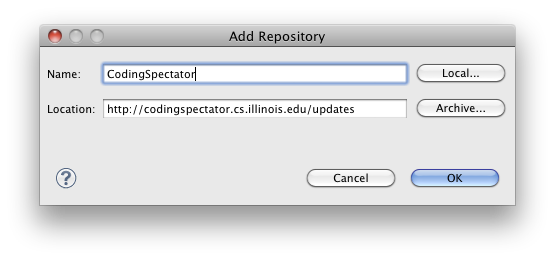
\includegraphics{figs/add_site}
%
\end{figure}

\item After adding our update-site, select the \codspec\ features:

\begin{figure}
%
\centering
%
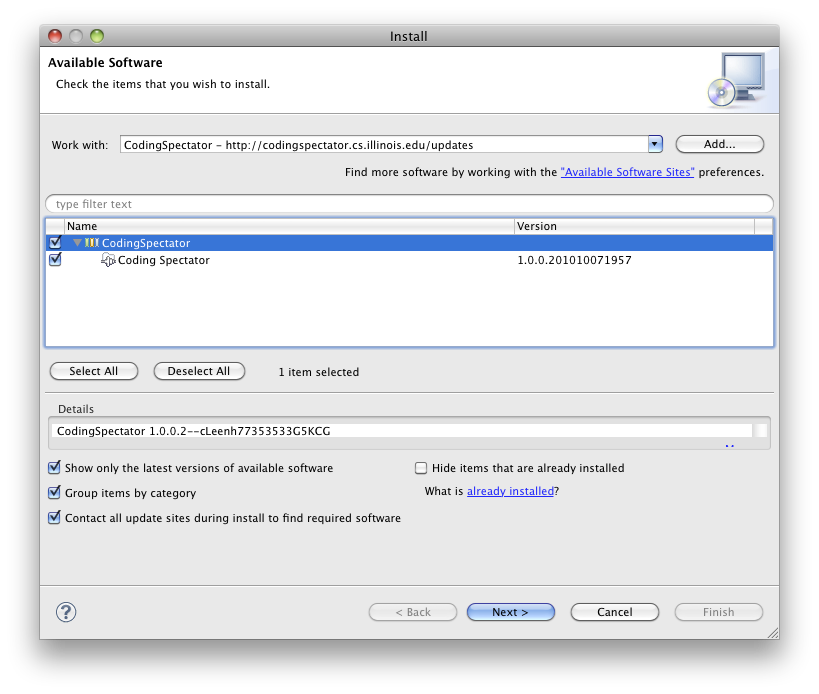
\includegraphics{figs/select_features}
%
\end{figure}

\item Click \uiref{Next} to proceed.

\item You will now be presented with the \uiref{Install Details} dialog window
listing the items that will be installed. Ensure that our \codspec\ plug-in and
all its components are selected. Click \uiref{Next}.

\item You will now be presented with the \uiref{Review Licenses} dialog window
detailing the licenses of the plug-ins that will be installed. Take a moment to
review them, and if you agree, proceed by clicking \uiref{Finish}.

\item There will be a dialog (like the one below) warning you that you are
installing unsigned content. Do not be alarmed by this; our plug-ins are simply
not signed for this research study. Click \uiref{OK}.

\begin{figure}
%
\centering
%
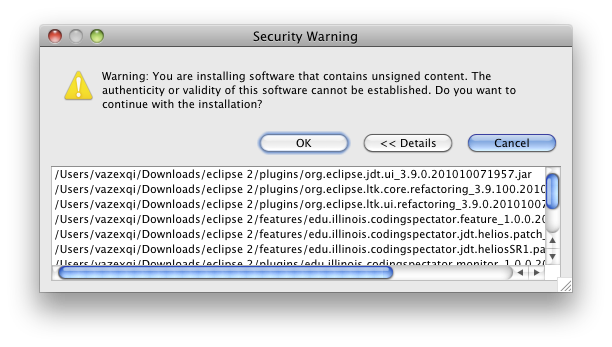
\includegraphics{figs/warning}
%
\end{figure}

\item A dialog will pop-up asking you to restart Eclipse after the software
updates. Click \uiref{Restart Now}. Please do \textbf{not} use the other options
on that dialog.

\item You have successfully installed our plug-in.
%
\end{enumerate}
%
\section{Running our plug-in}
%
Our plug-in is a non-intrusive extension that monitors your coding activities
inside Eclipse. It will run in the background and will not interfere with your
coding routines except for the occasional dialog asking you to upload your data.
Your data will be uploaded to a secure TSG server that only the researchers have
access to.

\infonote{Our plug-in will monitor for programming behavior in \textbf{all}
workspaces that you create using that particular Eclipse instance. As detailed
in the consent form (\url{https://illinois.edu/fb/sec/9663171}), the plug-in
will record certain code development activities that are performed in the
workspace and store that information. In addition, the plug-in might collect
some code snippets to provide more context to the activities that are being
performed.

If you have sensitive data that you do not wish the plug-in to collect, you
would need to install two instances of Eclipse: one with our plug-in and one
\textbf{without} our plug-in.

Please feel free to talk to us if you have any questions and concerns about your
privacy. We can work our a suitable compromise.}
%
\section{Automatic upload of data}

\textbf{Once a day (at most)}, during the initial startup of Eclipse, you might
be presented with the dialog box below asking you to upload your data. Please
provide your UIUC netid and AD password when prompted.

\begin{figure}
%
\centering
%
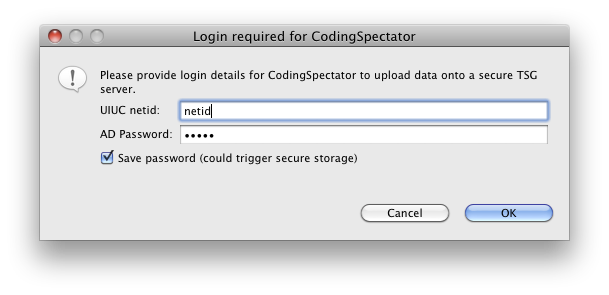
\includegraphics{figs/login}
%
\end{figure}

If you provide the wrong username/password, our plug-in will prompt you again:

\begin{figure}
%
\centering
%
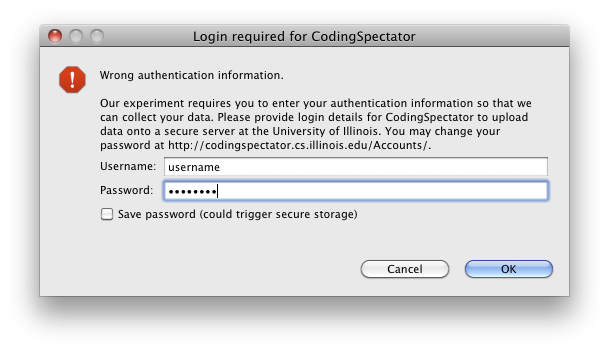
\includegraphics{figs/prompt}
%
\end{figure}

If you wish, you may also click on the \uiref{Save password (could trigger
secure storage)} checkbox. This will ask Eclipse to store your username and
password using its underlying Secure Storage mechanism
(\url{http://help.eclipse.org/helios/index.jsp?topic=/org.eclipse.platform.doc.isv/guide/secure_storage_dev.htm}).
If you decide to save your password, it will proceed to ask you to create a
master password. Please follow the instructions on screen as they are
OS-dependent.

Additionally, if you decide to save your password, on subsequent uploads of our
plug-in, you will no longer see the dialog above but one of the following ones:

\begin{figure}
%
\centering
%
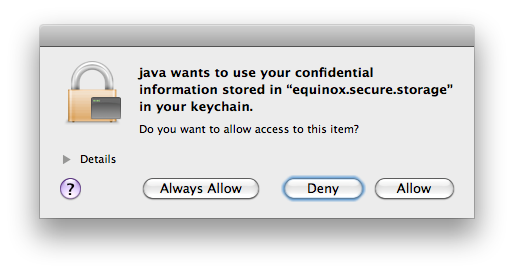
\includegraphics{figs/keychain}
%
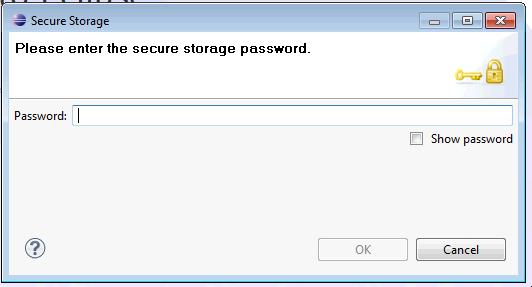
\includegraphics{figs/windows}
%
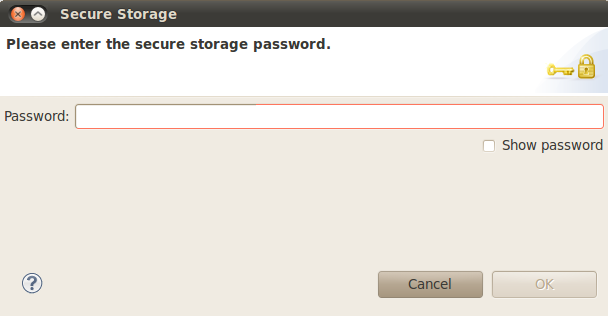
\includegraphics{figs/LinuxMasterPasswordDialog}
%
\end{figure}

Please enter the \textbf{master password} that you have created (\textbf{not}
your AD password) when prompted by the Secure Storage dialog box.

\section{Manual upload of data}

You may also trigger the data upload manually. We provide this facility because,
occasionally, it might not be convenient to upload the data during the startup
of Eclipse.

To invoke the manual uploading of your data, you can go to \uiref{Window >
Preferences} (on Linux and Windows) or \uiref{Eclipse > Preferences...} (on Mac
OS X). Click on the \uiref{\codspec} section.

\begin{figure}
%
\centering
%
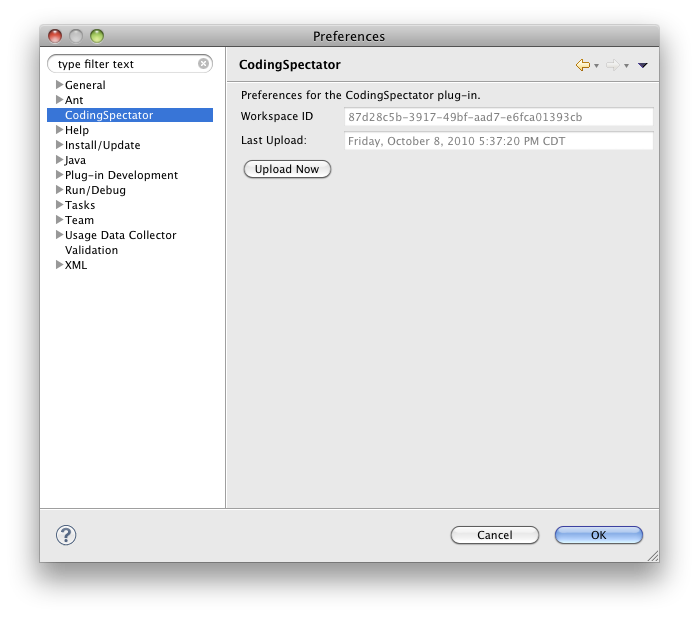
\includegraphics{figs/preferences}
%
\end{figure}

In that preference pane, you will see:

\begin{enumerate}
%
\item a special ID that we use to identify the workspace that you are working on
%
\item the date and time of your last upload
%
\item an \uiref{Upload Now} button that you can invoke to upload your data
%
\end{enumerate}

\section{Developing Photran plug-ins}

\warnnote{This section \uiref{Developing Photran plug-ins} is important. Please
read and follow the instructions carefully. The mechanism for doing this might
seem complicated at first but it is a direct result of the Eclipse ecosystem and
its conventions. If you have any questions, we are available to help.}

As part of the final project for CS427, you will be expected to develop a
plug-in for Photran. There is an additional step that you need to perform before
\textbf{running/debugging/testing} your Photran instance: you need to modify
your launch configuration so that it does \textbf{not} launch our \codspec\
plug-in.  This prevents it from popping-up the dialog window each time you
run/debug/test Photran and prevents it from spuriously logging your data.

\begin{enumerate}
%
\item Create a new \uiref{Target Platform} configuration. Go to \uiref{Window >
Preference} (on Linux and Windows) or \uiref{Eclipse > Preferecences...} (on Mac
OS X). Type in \uiref{target} in the search dialog to shorten the list to bring
up the \uiref{Target Platform} preferences.  \item Click on \uiref{Target
Platform} on the list on the left.

\begin{figure}
%
\centering
%
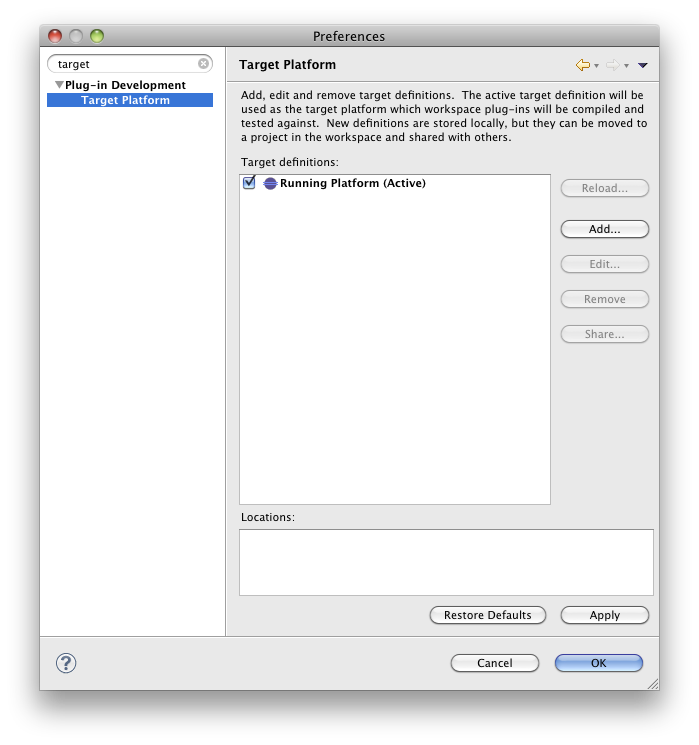
\includegraphics{figs/target_step1}
%
\end{figure}
%
\item Click \uiref{Add} on the right hand side of the window.
%
\item In the dialog that appears, select the second option \uiref{Default:
Default target for running platform}.

\begin{figure}
%
\centering
%
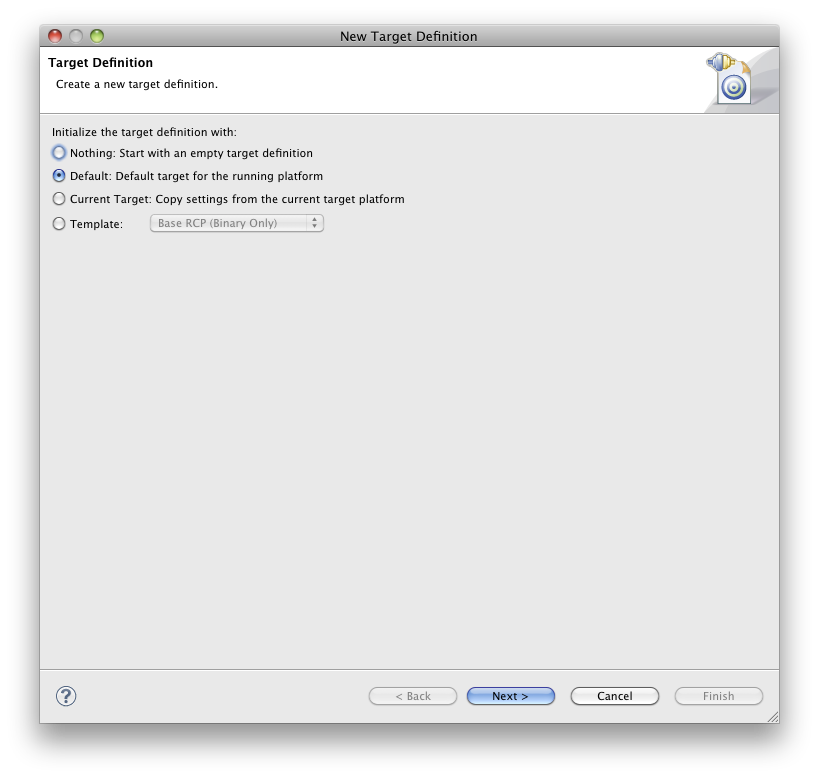
\includegraphics{figs/target_step2}
%
\end{figure}

\item Click \uiref{Next}.
%
\item In the dialog that appears, put \uiref{\codspec} for the new name in
textfield at the top.
%
\item Click on the \uiref{Content} tab. Type in "edu.illinois" to narrow down
the list of plug-ins. \textbf{Deselect} the following (and only the following):

\begin{enumerate} \item edu.illinois.codingspectator.monitor.ui

\begin{figure}
%
\centering
%
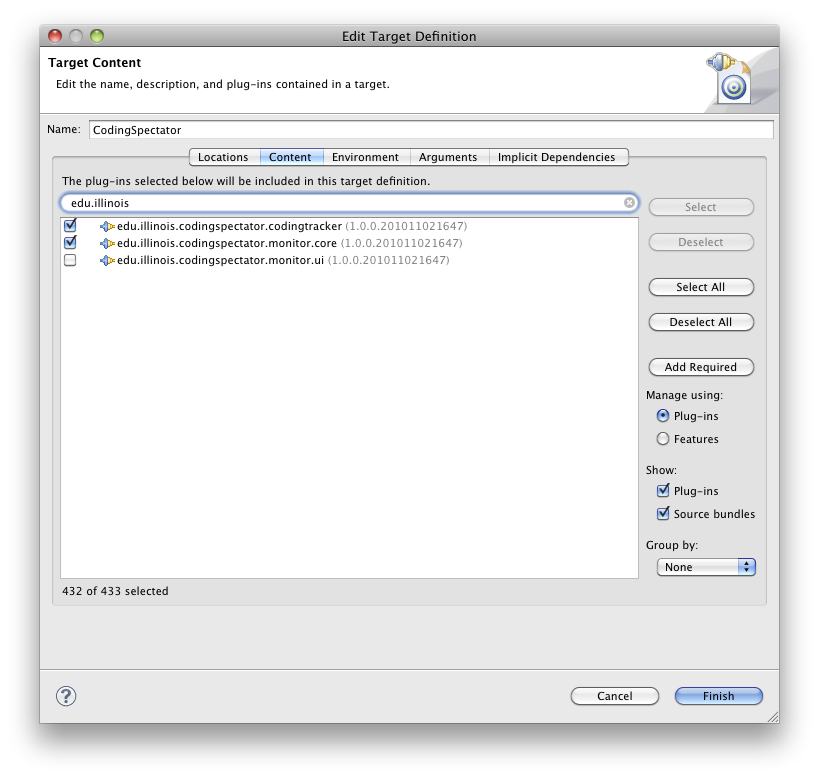
\includegraphics{figs/target_step3}
%
\end{figure}
%
\item Click \uiref{Finish}.
%
\item In the preferences window, \textbf{check} the \uiref{\codspec\ Target
Platform} that you have just created.

\begin{figure}
%
\centering
%
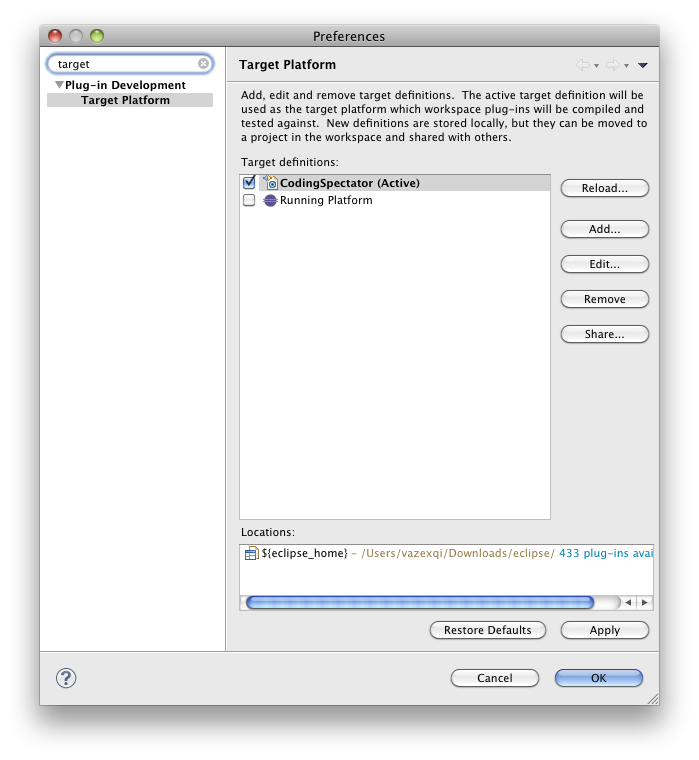
\includegraphics{figs/target_step4}
%
\end{figure}
%
\item Click \uiref{OK}.
%
\end{enumerate}
%
\end{enumerate}
%
\section{Updating our plug-in}

During this research study, we might require you to update our plug-in. Should
this become necessary, we will contact you via e-mail to upgrade the plug-in.
This is a simple process that you can perform by going to \uiref{Help > Check
for Updates} in the Eclipse application.

\begin{figure}
%
\centering
%
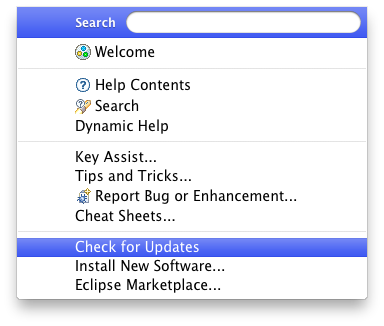
\includegraphics{figs/updates}
%
\end{figure}
%
\section{Uninstalling our plug-in}

\begin{enumerate}
%
\item You can uninstall our plug-in through the \uiref{About Eclipse...} dialog.
You can invoke this dialog (shown below) by going to \uiref{Eclipse > About
Eclipse...} on OS X or through \uiref{Help > About Eclipse...} on Linux and
Windows.

\begin{figure}
%
\centering
%
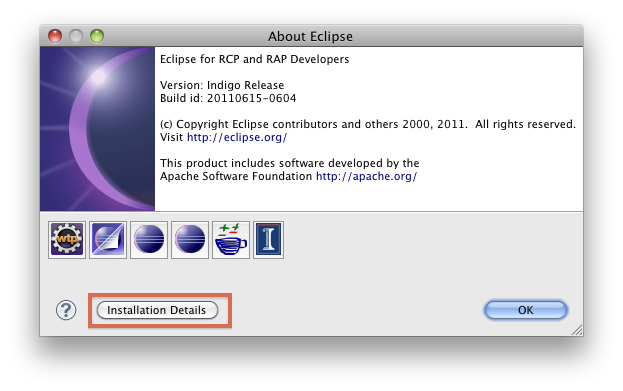
\includegraphics{figs/uninstall_step1}
%
\end{figure}
%
\item In that dialog, click on the \uiref{Installation Details} button. A new
dialog (shown below) should appear. The list of plug-ins installed might be
different from the image below depending on what other plug-ins you have
installed.

\begin{figure}
%
\centering
%
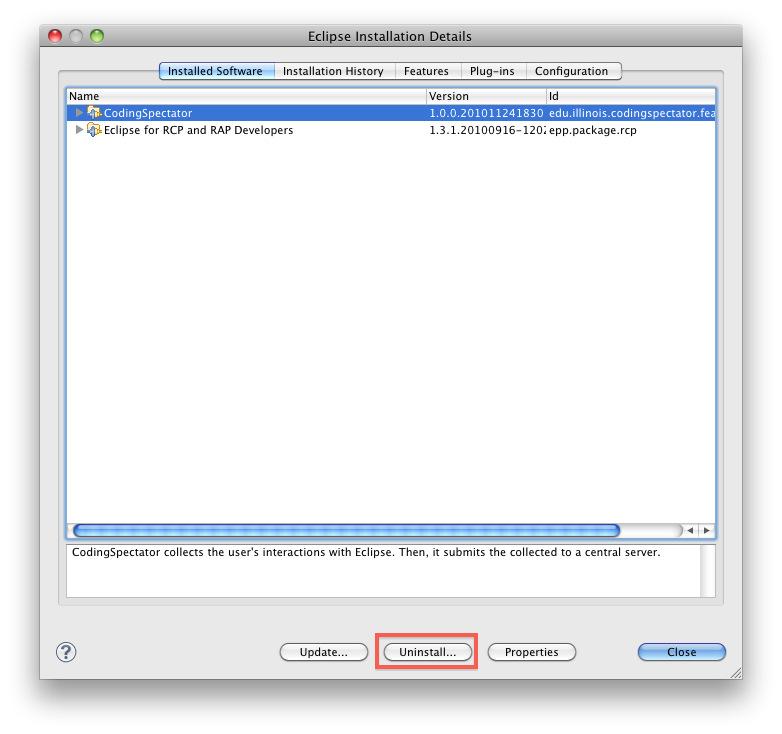
\includegraphics{figs/uninstall_step2}
%
\end{figure}
%
\item Click on \uiref{\codspec} from the list to select it. Then click on the
\uiref{Uninstall...} button.
%
\item Eclipse will calculate the dependencies and uninstallation validity. After
a while, it will show the dialog below.

\begin{figure}
%
\centering
%
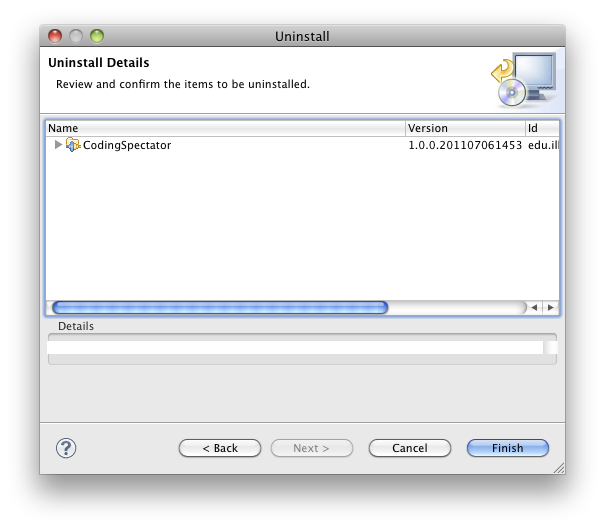
\includegraphics{figs/uninstall_step3}
%
\end{figure}
%
\item Click \uiref{Finish}
%
\item Eclipse will proceed to uninstall \codspec. After a while, a dialog will
pop-up asking if you would like to restart Eclipse for the changes to take
effect. Click \uiref{Restart Now}.

\begin{figure}
%
\centering
%
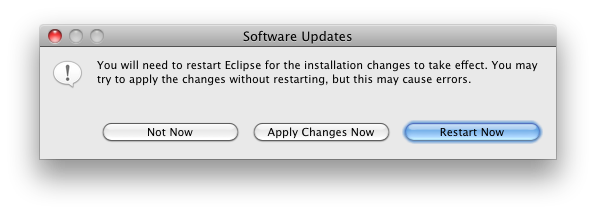
\includegraphics{figs/uninstall_step4}
%
\end{figure}
%
\end{enumerate}
%
\end{document}

